\subsection{External Interface Requirements}
\subsubsection{User Interfaces}
\subsubsection{Hardware Interfaces}
\subsubsection{Software Interfaces}
\subsubsection{Communication Interfaces}
\subsection{Functional Requirements}
This chapter provides a comprehensive overview of the system's use cases, detailing the various interactions between Users and the system.
Use Case Diagrams, detailed Use Case Descriptions, Sequence Diagrams and Requirement Mapping are provided for each use case.
\subsubsection{Use Case Diagrams}
\begin{figure}[H]
    \centering
    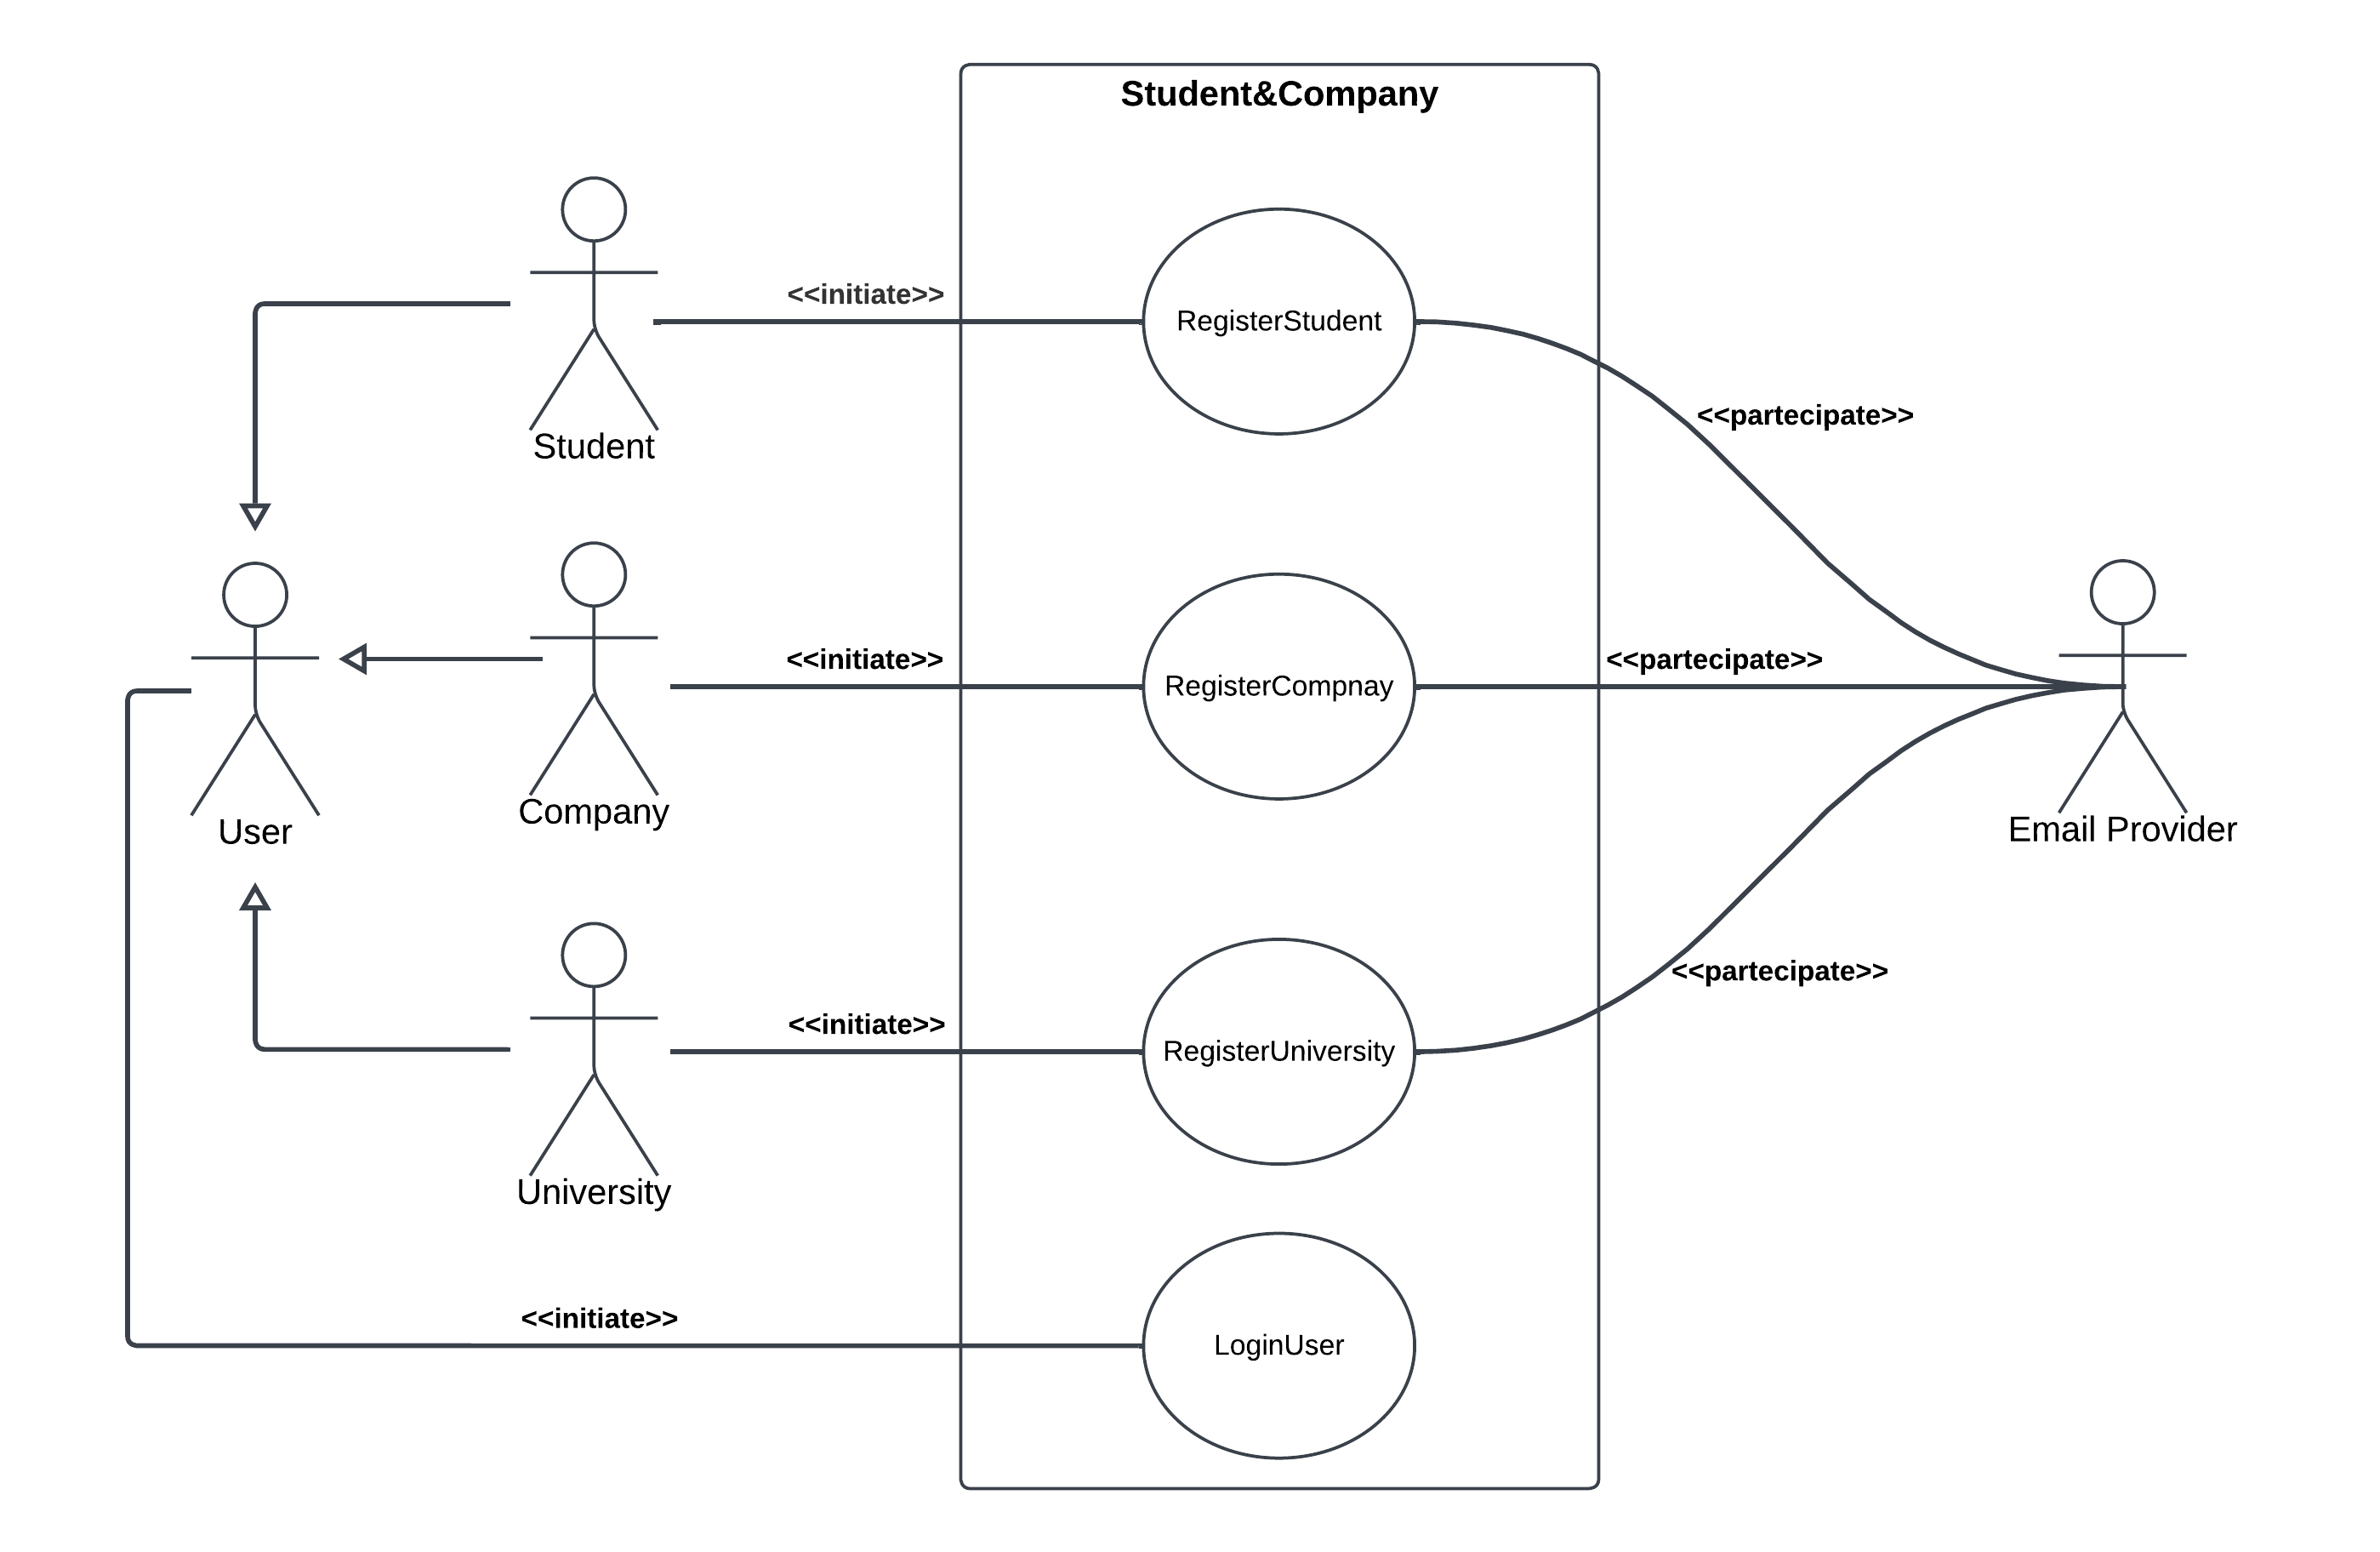
\includegraphics[width=1 \textwidth]{Diagrams/UseDiagrams/UserRegistrationUseCase.png}
    \caption{User Registration Use Case Diagram}
    \label{fig:UserRegistrationUseCaseDiagram}
\end{figure}
\begin{figure}[H]
    \centering
    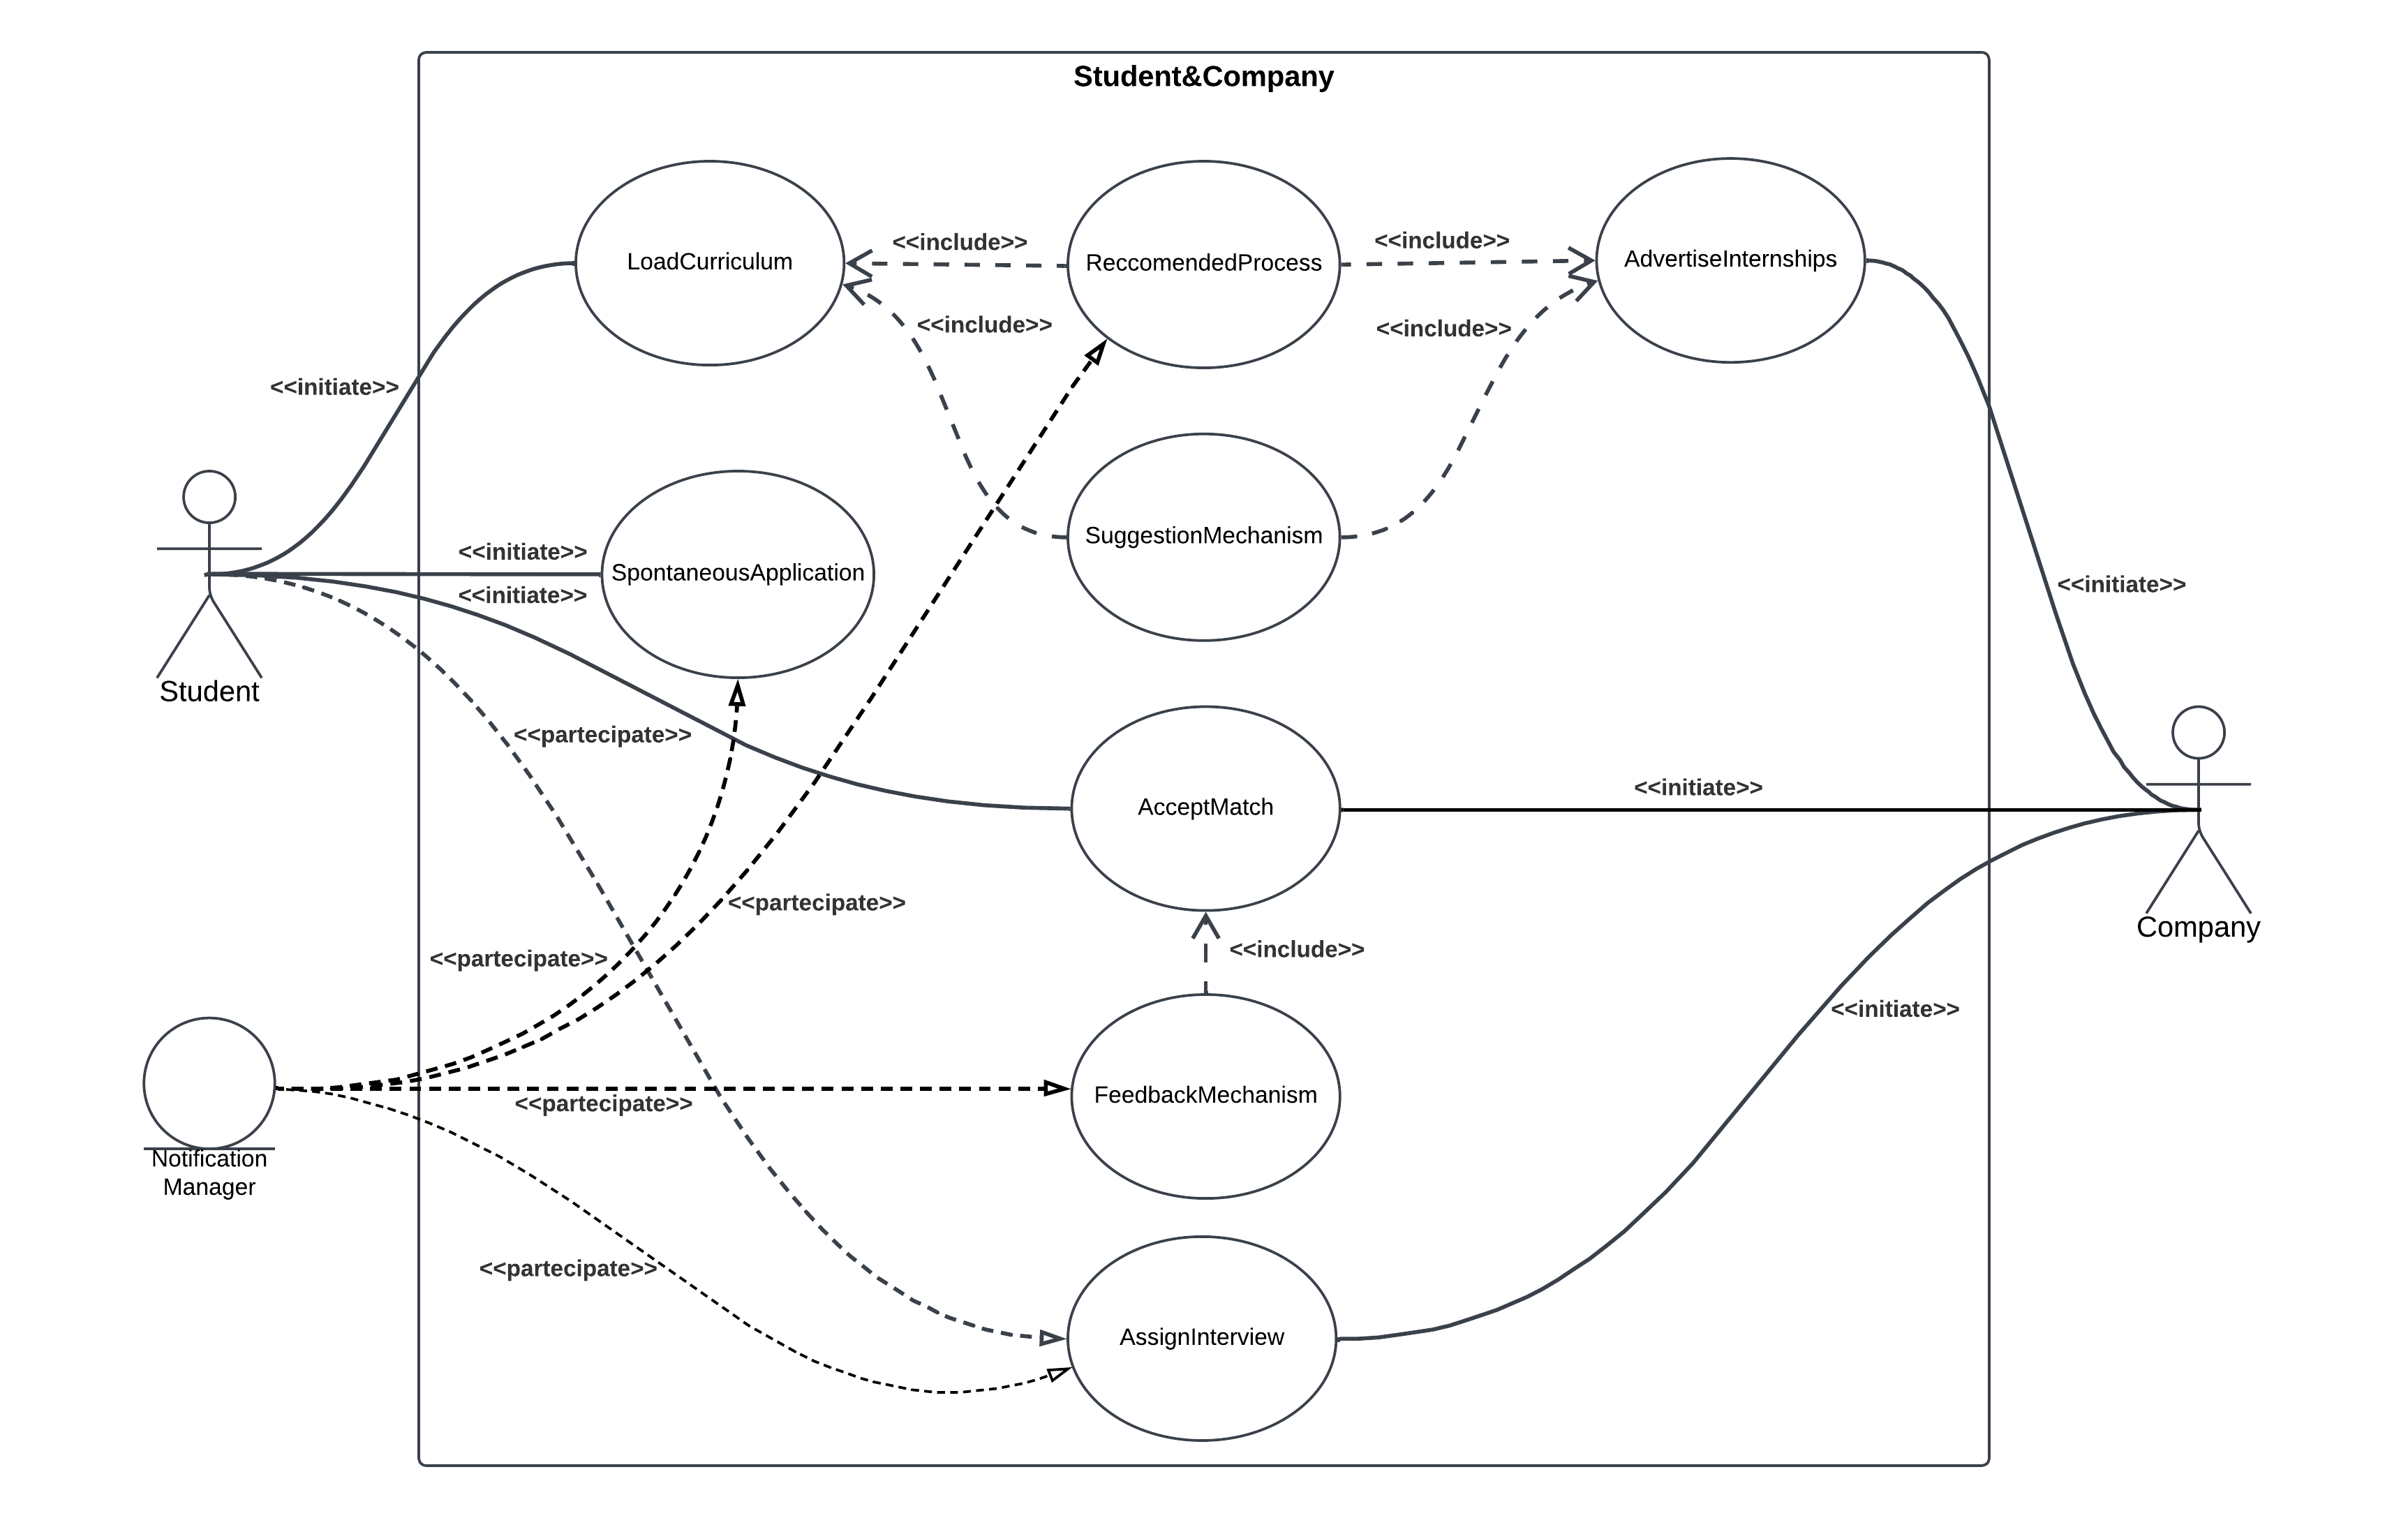
\includegraphics[width=1 \textwidth]
    {Diagrams/UseDiagrams/Student Company Use Case.png}
    \caption{Student and Company Use Case Diagram}
    \label{fig:StudentCompanyUseCaseDiagram}
\end{figure}
\begin{figure}[H]
    \centering
    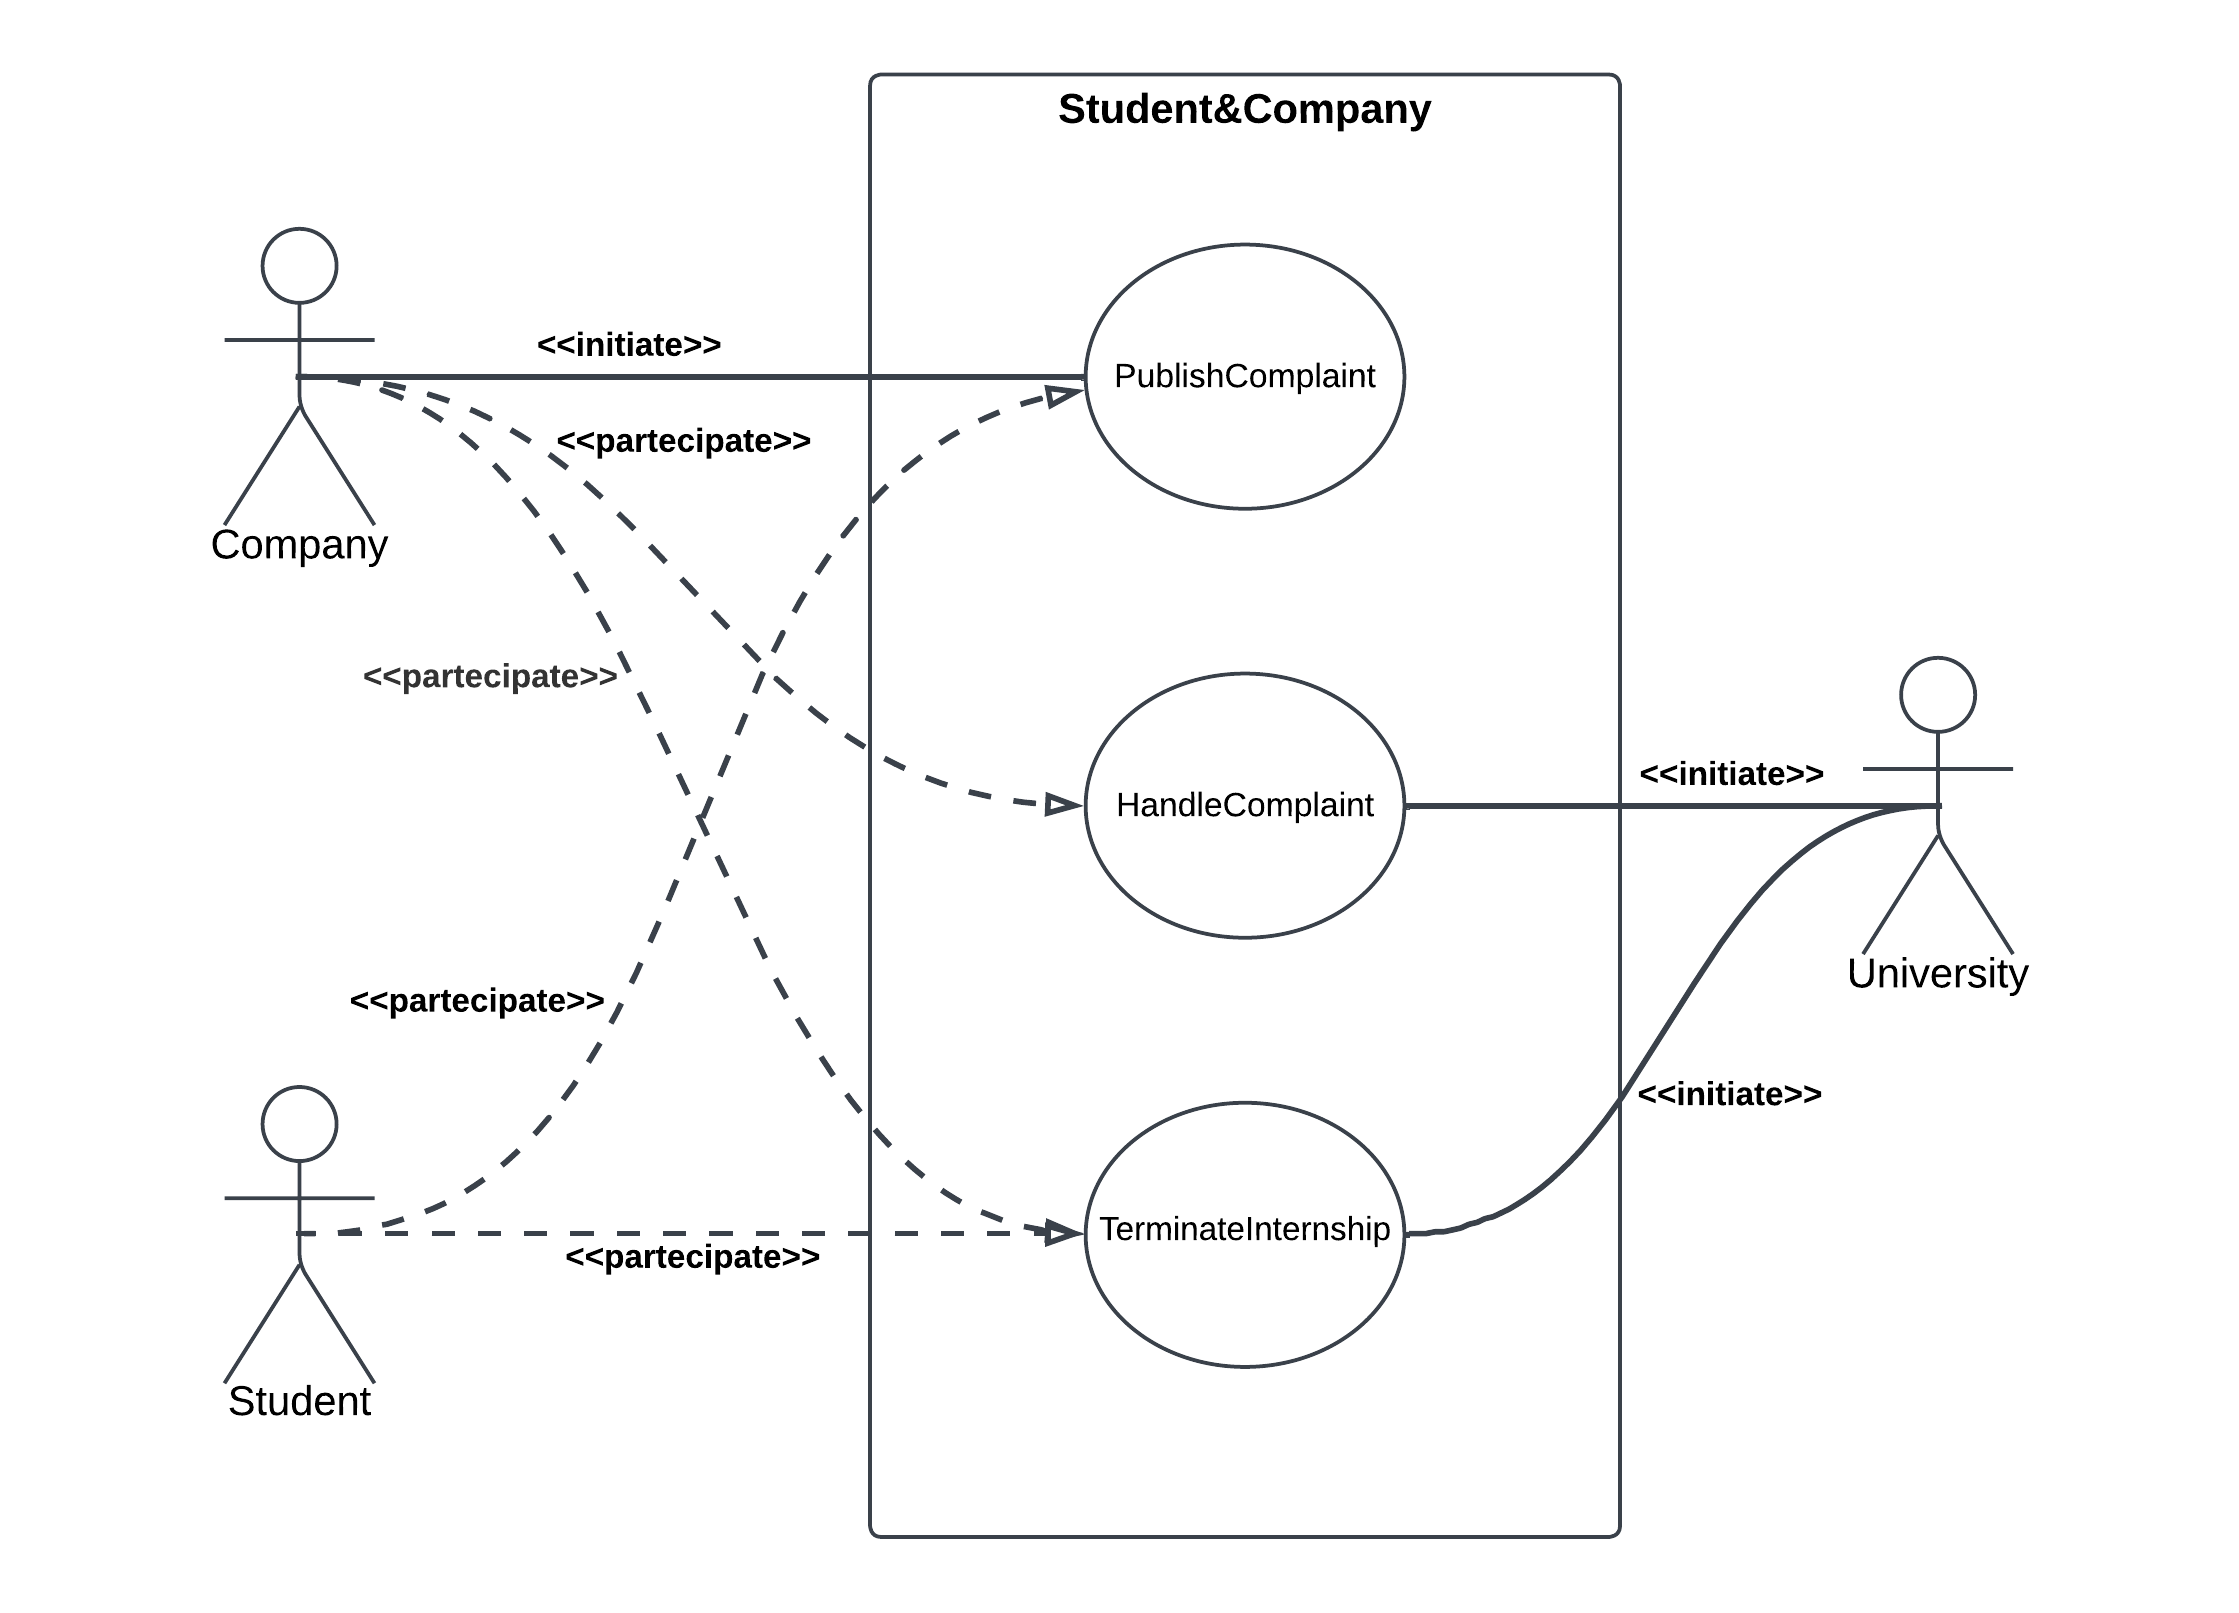
\includegraphics[width=1 \textwidth]{Diagrams/UseDiagrams/UniversityUseCaseDiagram.png}
    \caption{University and Complaint Use Case Diagram}
    \label{fig:UniveristyUseCaseDiagram}
\end{figure}


\subsubsection{Use Cases}

\begin{table}[H]
    \centering
    \begin{tabular}{|p{3cm}|p{12cm}|}
    \hline
    \multicolumn{2}{|c|}{\textbf{RegisterStudent}} \\ \hline
    Actor & 
    \begin{itemize}
        \item Student
        \item Email Provider
    \end{itemize} \\ \hline
    Entry Condition & The user is not logged in. \\ \hline
    Event Flow & 
    \begin{enumerate}         
        \item The student selects the “Sign up” option.
        \item The platform open the sign-up page.
        \item The student selects the “Student” option, provides the required information (name, surname, date of birth, institutional email, optionally personal email, password, University name among those available) and click the “Sign Up” button.
        \item The platform validates the email and checks if it is unique.
        \item The platform registers the Student and sends a confirmation email to the provided email address through the Email Provider.
        \item The Student confirms the registration by clicking on the link in the email.
        \item The platform confirms the registration and activates the account.
        \item The Student is redirected to the platform's homepage.
    \end{enumerate} \\ \hline
    Exit Condition & The Student is registered and logged in. \\ \hline
    Exception & 
    \begin{itemize}
        \item The Student provides incorrect information.
        \item The Email Provider fails to send the confirmation email.
        \item The Student does not confirm the registration.
        \item The email is already in use.
    \end{itemize} \\ \hline
    \end{tabular}
    \caption{[UC1]: Student registration use case}
    \label{tab:UC1}
\end{table}
\clearpage
\begin{table}[H]
    \centering
    \begin{tabular}{|p{3cm}|p{12cm}|}
    \hline
    \multicolumn{2}{|c|}{\textbf{RegisterCompany}} \\ \hline
    Actor & 
    \begin{itemize}
        \item Company
        \item Email Provider
    \end{itemize} \\ \hline
    Entry Condition & The user is not logged in \\ \hline
    Event Flow &
    \begin{enumerate}         
        \item The company selects the “Sign up” option.
        \item The platform open the sign-up page.
        \item The company selects the “Company” option, provides the required information (Company name, Company headquarters address, VAT number, email, and password) and click the “Sign Up” button.
        \item The platform sends a confirmation email to the provided email address through the Email Provider.
        \item The Company confirms the registration by clicking on the link in the email.
        \item The platform validates the VAT number and checks if it is unique.
        \item The platform confirms the registration and activates the account.
        \item The Company is redirected to the platform's homepage.
    \end{enumerate} \\ \hline
    Exit Condition & The Company is registered and logged in. \\ \hline
    Exception & 
    \begin{itemize}
        \item The Company provides incorrect information.
        \item The Email Provider fails to send the confirmation email.
        \item The Company does not confirm the registration.
        \item The VAT number is already in use.
    \end{itemize} \\ \hline
    \end{tabular}
    \caption{[UC2]: Company registration use case}
    \label{tab:UC2}
\end{table}

\begin{table}[H]
    \centering
    \begin{tabular}{|p{3cm}|p{12cm}|}
    \hline
    \multicolumn{2}{|c|}{\textbf{RegisterUniversity}} \\ \hline
    Actor & 
    \begin{itemize}
        \item University
        \item Email Provider
    \end{itemize} \\ \hline
    Entry Condition & The user is not logged in. \\ \hline
    Event Flow &
    \begin{enumerate}         
        \item The university selects the “Sign up” option.
        \item The platform open the sign-up page.
        \item The university selects the “University” option, provides the required information (University Name, University description, VAT number, email of the University office that will manage the internship program, and password) and click the “Sign Up” button.
        \item The platform sends a confirmation email to the provided email address through the Email Provider.
        \item The platform confirms the registration by clicking on the link in the email.
        \item The platform validates the VAT number and checks if it is unique.
        \item The platform confirms the registration and activates the account.
        \item The University is redirected to the platform's homepage.
    \end{enumerate} \\ \hline
    Exit Condition & The University is registered and logged in.\\ \hline
    Exceptions &
    \begin{itemize}
        \item The University provides incorrect information.
        \item The Email Provider fails to send the confirmation email.
        \item The University does not confirm the registration.
        \item The VAT number is already in use.
    \end{itemize} \\ \hline
    \end{tabular}
    \caption{[UC3]: University registration use case}
    \label{tab:UC3}
\end{table}

\begin{table}[H]
    \centering
    \begin{tabular}{|p{3cm}|p{12cm}|}
    \hline
    \multicolumn{2}{|c|}{\textbf{LoginUser}} \\ \hline
    Actor & 
    \begin{itemize}
        \item User
    \end{itemize}\\ \hline
    Entry Condition & \\ \hline
    Event Flow &
    \begin{enumerate}         
        \item The User selects the “Sign in” option.
        \item The platform open the sign-in page.
        \item The user provides their email and password.
        \item The platform validates the credentials.
        \item The platform confirms the credentials and logs in the User.
        \item The User is redirected to the platform's homepage.
    \end{enumerate} \\ \hline
    Exit Condition & The User is logged in. \\ \hline
    Exceptions &
    \begin{itemize}
        \item The User provides incorrect email or password.
    \end{itemize} \\ \hline
    \end{tabular}
    \caption{[UC4]: User login use case}
    \label{tab:UC4}
\end{table}

\begin{table}[H]
    \centering
    \begin{tabular}{|p{3cm}|p{12cm}|}
    \hline
    \multicolumn{2}{|c|}{\textbf{LoadCurriculum}} \\ \hline
    Actor & 
    \begin{itemize}
        \item Student
    \end{itemize}\\ \hline
    Entry Condition & \\ \hline
    Event Flow &
    \begin{enumerate}         
        \item The Student selects the “Upload CV” option.
        \item The platform open the Curriculum page.
        \item The Student fills the form with the required information (current level of education, known languages, technical skills, a photo of himself, a brief description of his interests and hobbies etc…) and click the “Submit CV” button.
        \item The platform publishes the CV.
        \item The platform generates a list of matching internships based on the CV.
        \item The platform provides feedback and suggestions to improve the CV.
        \item The Student is redirected to his account page.
    \end{enumerate} \\ \hline
    Exit Condition & The Student's CV is uploaded, and the Student is redirected to his account page. \\ \hline
    Exception & 
    \begin{itemize} 
        \item The Student provides invalid or partial information.
        \item The Student exits the page before submitting the CV.
    \end{itemize} \\ \hline
    \end{tabular}
    \caption{[UC5]: Student uploads Curriculum use case}
    \label{tab:UC5}
\end{table}

\begin{table}[H]
    \centering
    \begin{tabular}{|p{3cm}|p{12cm}|}
    \hline
    \multicolumn{2}{|c|}{\textbf{AdvertiseInternships}} \\ \hline
    Actor & \\ \hline
    Entry Condition & \\ \hline
    Event Flow &
    \begin{enumerate}         
        \item Something
        \item Something
    \end{enumerate} \\ \hline
    Exit Condition & \\ \hline
    Exception & 
    \begin{itemize}        
        \item
    \end{itemize} \\ \hline
    \end{tabular}
    \caption{[UC6]: Internships advertising use case}
    \label{tab:UC6}
\end{table}

\begin{table}[H]
    \centering
    \begin{tabular}{|p{3cm}|p{12cm}|}
    \hline
    \multicolumn{2}{|c|}{\textbf{SpontaneousApplication}} \\ \hline
    Actor & \\ \hline
    Entry Condition & \\ \hline
    Event Flow &
    \begin{enumerate}         
        \item Something
        \item Something
    \end{enumerate} \\ \hline
    Exit Condition & \\ \hline
    Exception & 
    \begin{itemize}       
        \item     
    \end{itemize} \\ \hline
    \end{tabular}
    \caption{[UC7]: Student Spontaneous Application submission use case}
    \label{tab:UC7}
\end{table}

\begin{table}[H]
    \centering
    \begin{tabular}{|p{3cm}|p{12cm}|}
    \hline
    \multicolumn{2}{|c|}{\textbf{AcceptMatch}} \\ \hline
    Actor & \\ \hline
    Entry Condition & \\ \hline
    Event Flow &      
    \begin{enumerate}         
        \item Something
        \item Something
    \end{enumerate} \\ \hline
    Exit Condition & \\ \hline
    Exception & 
    \begin{itemize}        
        \item     
    \end{itemize} \\ \hline
    \end{tabular}
    \caption{[UC8]: Company and Student Match use case}
    \label{tab:UC8}
\end{table}

\begin{table}[H]
    \centering
    \begin{tabular}{|p{3cm}|p{12cm}|}
    \hline
    \multicolumn{2}{|c|}{\textbf{RecommendedProcess}} \\ \hline
    Actor & \\ \hline
    Entry Condition & \\ \hline
    Event Flow &      
    \begin{enumerate}         
        \item Something
        \item Something
    \end{enumerate} \\ \hline
    Exit Condition & \\ \hline
    Exception & 
    \begin{itemize}     
        \item    
    \end{itemize} \\ \hline
    \end{tabular}
    \caption{[UC9]: Recommendation Process use case}
    \label{tab:UC9}
\end{table}

\begin{table}[H]
    \centering
    \begin{tabular}{|p{3cm}|p{12cm}|}
    \hline
    \multicolumn{2}{|c|}{\textbf{SuggestionMechanism}} \\ \hline
    Actor & \\ \hline
    Entry Condition & \\ \hline
    Event Flow &      
    \begin{enumerate}         
        \item Something
        \item Something
    \end{enumerate} \\ \hline
    Exit Condition & \\ \hline
    Exception & 
    \begin{itemize}        
        \item     
    \end{itemize} \\ \hline
    \end{tabular}
    \caption{[UC10]: Suggestion mechanism use case}
    \label{tab:UC10}
\end{table}

\begin{table}[H]
    \centering
    \begin{tabular}{|p{3cm}|p{12cm}|}
    \hline
    \multicolumn{2}{|c|}{\textbf{AssignInterview}} \\ \hline
    Actor & \\ \hline
    Entry Condition & \\ \hline
    Event Flow &      
    \begin{enumerate}         
        \item Something
        \item Something
    \end{enumerate} \\ \hline
    Exit Condition & \\ \hline
    Exception & 
    \begin{itemize}         
        \item     
    \end{itemize} \\ \hline
    \end{tabular}
    \caption{[UC11]: Interview assignment use case}
    \label{tab:UC11}
\end{table}

\begin{table}[H]
    \centering
    \begin{tabular}{|p{3cm}|p{12cm}|}
    \hline
    \multicolumn{2}{|c|}{\textbf{PublishComplaint}} \\ \hline
    Actor & \\ \hline
    Entry Condition & \\ \hline
    Event Flow &      
    \begin{enumerate}         
        \item Something
        \item Something
    \end{enumerate} \\ \hline
    Exit Condition & \\ \hline
    Exception & 
    \begin{itemize}       
        \item   
    \end{itemize} \\ \hline
    \end{tabular}
    \caption{[UC12]: Complaint publication use case}
    \label{tab:UC12}
\end{table}

\begin{table}[H]
    \centering
    \begin{tabular}{|p{3cm}|p{12cm}|}
    \hline
    \multicolumn{2}{|c|}{\textbf{HandleComplaint}} \\ \hline
    Actor & \\ \hline
    Entry Condition & \\ \hline
    Event Flow &      
    \begin{enumerate}         
        \item Something
        \item Something
    \end{enumerate} \\ \hline
    Exit Condition & \\ \hline
    Exception & 
    \begin{itemize}         
        \item    
    \end{itemize} \\ \hline    
    \end{tabular}
    \caption{[UC13]: Complaint management use case}
    \label{tab:UC13}
\end{table}

\begin{table}[H]
    \centering
    \begin{tabular}{|p{3cm}|p{12cm}|}
    \hline
    \multicolumn{2}{|c|}{\textbf{TerminateInternship}} \\ \hline
    Actor & \\ \hline
    Entry Condition & \\ \hline
    Event Flow &      
    \begin{enumerate}         
        \item Something
        \item Something
    \end{enumerate} \\ \hline
    Exit Condition & \\ \hline
    Exception & 
    \begin{itemize}         
        \item      
    \end{itemize} \\ \hline  
    \end{tabular}
    \caption{[UC14]: Internship termination use case}
    \label{tab:UC14}
\end{table}


\subsubsection{Sequence Diagrams}

\clearpage
\subsubsection{Requirements Mapping}

\begin{table}[H]
    \centering
    \begin{tabular}{|p{15cm}|}
         \hline
        \textbf{G1:} Companies would like to advertise the internships they offer. \\ \hline
        \begin{itemize}
            \item[\texttt{[D1]}] Students and Companies provide the Platform with correct and truthful information.
            \item[\texttt{[D2]}] Companies remove published Internship if they are no longer available.
            \item[\texttt{[D3]}] Students, Companies, and Universities receive every notification.
            \item[\texttt{[D4]}] Students, Companies, and Universities have a working internet connection.
        \end{itemize} \\ \hline
        \begin{itemize}
            \item[\texttt{[R1]}] The platform shall allow any unregistered students to register by providing personal information and selecting their University.
            \item[\texttt{[R2]}] The platform shall allow any companies to register by providing company information.
            \item[\texttt{[R3]}] The platform shall allow any universities to register by providing university information.
            \item[\texttt{[R4]}] The platform shall allow Users to log in using their email and password.
            \item[\texttt{[R5]}] The platform shall send notifications to Users when relevant events occur.
            \item[\texttt{[R6]}] The platform shall allow Companies to create and publish Internship offers specifying details.
            \item[\texttt{[R7]}] The platform shall allow Companies to terminate their Internship offers at their own discretion.
            \item[\texttt{[R9]}] The platform shall allow Students to view and navigate all available Internships.
        \end{itemize} \\ \hline
    \end{tabular}
    \caption{Goal 1 mapping}
    \label{tab:G1}
\end{table}
\clearpage
\begin{table}[H]
    \centering
    \begin{tabular}{|p{15cm}|}
         \hline
        \textbf{G2:} Students would like to autonomously candidate for available internships. \\ \hline
        \begin{itemize}
            \item[\texttt{[D1]}] Students and Companies provide the Platform with correct and truthful information. 
            \item[\texttt{[D2]}] Companies remove published Internship if they are no longer available.
            \item[\texttt{[D3]}] Students, Companies, and Universities receive every notification.
            \item[\texttt{[D4]}] Students, Companies, and Universities have a working internet connection.
        \end{itemize} \\ \hline
        \begin{itemize}
            \item[\texttt{[R1]}] The platform shall allow any unregistered students to register by providing personal information and selecting their University.
            \item[\texttt{[R2]}] The platform shall allow any companies to register by providing company information.
            \item[\texttt{[R3]}] The platform shall allow any universities to register by providing university information.
            \item[\texttt{[R4]}] The platform shall allow Users to log in using their email and password.
            \item[\texttt{[R5]}] The platform shall send notifications to Users when relevant events occur.
            \item[\texttt{[R6]}] The platform shall allow Companies to create and publish Internship offers specifying details.
            \item[\texttt{[R7]}] The platform shall allow Companies to terminate their Internship offers at their own discretion.
            \item[\texttt{[R9]}] The platform shall allow Students to view and navigate all available Internships.
            \item[\texttt{[R10]}] The platform shall enable Students to submit Spontaneous Applications to Internships they choose.
            \item[\texttt{[R13]}] The platform shall allow Students to monitor the status of their Spontaneous Applications.
            \item[\texttt{[R18]}] The platform shall allow Companies to accept a Spontaneous Application.
        \end{itemize} \\ \hline
    \end{tabular}
    \caption{Goal 2 mapping}
    \label{tab:G2}
\end{table}

\begin{table}[H]
    \centering
    \begin{tabular}{|p{15cm}|}
        \hline
        \textbf{G3:} Students would like to be matched with internships they might be interested in. \\ \hline
        \begin{itemize}
            \item[\texttt{[D1]}] Students and Companies provide the Platform with correct and truthful information.
            \item[\texttt{[D2]}] Companies remove published Internship if they are no longer available.
            \item[\texttt{[D3]}] Students, Companies, and Universities receive every notification.
            \item[\texttt{[D4]}] Students, Companies, and Universities have a working internet connection.
        \end{itemize} \\ \hline
        \begin{itemize}
            \item[\texttt{[R1]}] The platform shall allow any unregistered students to register by providing personal information and selecting their University.
            \item[\texttt{[R2]}] The platform shall allow any companies to register by providing company information.
            \item[\texttt{[R3]}] The platform shall allow any universities to register by providing university information.
            \item[\texttt{[R4]}] The platform shall allow Users to log in using their email and password.
            \item[\texttt{[R5]}] The platform shall send notifications to Users when relevant events occur.
            \item[\texttt{[R6]}] The platform shall allow Companies to create and publish Internship offers specifying details.
            \item[\texttt{[R7]}] The platform shall allow Companies to terminate their Internship offers at their own discretion.
            \item[\texttt{[R8]}] The platform shall provide Students with Matches automatically obtained by the Recommendation Process. 
            \item[\texttt{[R11]}] The platform shall allow Students to submit their CV.
            \item[\texttt{[R14]}] The platform shall allow Students to monitor the status of their Recommendation.
            \item[\texttt{[R15]}] The platform shall display to Students all the Internships found by the Recommendation Process.
            \item[\texttt{[R16]}] The platform shall display to Companies all the CVs of Matched Students obtained by the Recommendation Process.
            \item[\texttt{[R17]}] The platform shall allow Students and Companies to accept a Recommendation.
        \end{itemize} \\ \hline
    \end{tabular}
    \caption{Goal 3 mapping}
    \label{tab:G3}
\end{table}

\begin{table}[H]
    \centering
    \begin{tabular}{|p{15cm}|}
         \hline
        \textbf{G4:} Companies would like to perform interviews with suitable students. \\ \hline
        \begin{itemize}
            \item[\texttt{[D1]}] Students and Companies provide the Platform with correct and truthful information.
            \item[\texttt{[D2]}] Companies remove published Internship if they are no longer available.
            \item[\texttt{[D3]}] Students, Companies, and Universities receive every notification.
            \item[\texttt{[D4]}] Students, Companies, and Universities have a working internet connection.
        \end{itemize} \\ \hline
        \begin{itemize}
            \item[\texttt{[R1]}] The platform shall allow any unregistered students to register by providing personal information and selecting their University.
            \item[\texttt{[R2]}] The platform shall allow any companies to register by providing company information. 
            \item[\texttt{[R3]}] The platform shall allow any universities to register by providing university information.
            \item[\texttt{[R4]}] The platform shall allow Users to log in using their email and password.
            \item[\texttt{[R5]}] The platform shall send notifications to Users when relevant events occur.
            \item[\texttt{[R6]}] The platform shall allow Companies to create and publish Internship offers specifying details.
            \item[\texttt{[R17]}] The platform shall allow Students and Companies to accept a Recommendation.
            \item[\texttt{[R18]}] The platform shall allow Companies to accept a Spontaneous Application.
            \item[\texttt{[R19]}] The platform shall start a Selection Process only if both the Company and the Student have accepted the Recommendation.
            \item[\texttt{[R20]}] The platform shall start a Selection Process only if the Company has accepted the Spontaneous Application.
            \item[\texttt{[R21]}] The platform shall allow Companies to create Interviews.
            \item[\texttt{[R22]}] The platform shall allow Companies to submit Interviews to Students they have initiated a Selection Process with.
            \item[\texttt{[R23]}] The platform shall allow Students to answer Interview questions and submit them.
            \item[\texttt{[R24]}] The platform shall allow Companies to manually evaluate Interview submissions.
            \item[\texttt{[R25]}] The platform shall allow Students and Companies to monitor the status of their Interviews.
            \item[\texttt{[R26]}] The platform shall enable Companies to complete the Interview process by submitting the final outcome to each candidate.
        \end{itemize} \\ \hline
    \end{tabular}
    \caption{Goal 4 mapping}
    \label{tab:G4}
\end{table}

\begin{table}[H]
    \centering
    \begin{tabular}{|p{15cm}|}
        \hline
        \textbf{G5:} Students and companies would like to complain, communicate problems, provide information about an ongoing internship. \\ \hline
        \begin{itemize}
            \item[\texttt{[D1]}] Students and Companies provide the Platform with correct and truthful information.
            \item[\texttt{[D2]}] Companies remove published Internship if they are no longer available.
            \item[\texttt{[D3]}] Students, Companies, and Universities receive every notification.
            \item[\texttt{[D4]}] Students, Companies, and Universities have a working internet connection.
        \end{itemize} \\ \hline
        \begin{itemize}
            \item[\texttt{[R1]}] The platform shall allow any unregistered students to register by providing personal information and selecting their University.
            \item[\texttt{[R2]}] The platform shall allow any companies to register by providing company information.
            \item[\texttt{[R3]}] The platform shall allow any universities to register by providing university information.
            \item[\texttt{[R4]}] The platform shall allow Users to log in using their email and password.
            \item[\texttt{[R28]}] The platform shall enable Students to accept or reject an Internship Position Offer sent by a Company only if he previously passed the relative Interview.
            \item[\texttt{[R33]}] The platform shall provide a dedicated space for Students and Companies to exchange Communications about the current status of an ongoing Internship.
        \end{itemize} \\ \hline
    \end{tabular}
    \caption{Goal 5 mapping}
    \label{tab:G5}
\end{table}

\begin{table}[H]
    \centering
    \begin{tabular}{|p{15cm}|}
        \hline
        \textbf{G6:} Students and companies would like to be provided with suggestions about how to improve their submission. \\ \hline
        \begin{itemize}
            \item[\texttt{[D1]}] Students and Companies provide the Platform with correct and truthful information.
            \item[\texttt{[D4]}] Students, Companies, and Universities have a working internet connection.
        \end{itemize} \\ \hline
        \begin{itemize}
            \item[\texttt{[R1]}] The platform shall allow any unregistered students to register by providing personal information and selecting their University.
            \item[\texttt{[R2]}] The platform shall allow any companies to register by providing company information.
            \item[\texttt{[R3]}] The platform shall allow any universities to register by providing university information.
            \item[\texttt{[R4]}] The platform shall allow Users to log in using their email and password.
            \item[\texttt{[R6]}] The platform shall allow Companies to create and publish Internship offers specifying details.
            \item[\texttt{[R7]}] The platform shall allow Companies to terminate their Internship offers at their own discretion.
            \item[\texttt{[R12]}] The platform shall allow Students to modify their CV.
            \item[\texttt{[R29]}] The platform shall collect Feedback from both Students and Companies regarding the Recommendation Process.
            \item[\texttt{[R30]}] The platform shall provide Suggestions to Students on improving their CVs.
            \item[\texttt{[R31]}] The platform shall provide Suggestions to Companies on improving Internship descriptions.
        \end{itemize} \\ \hline
    \end{tabular}
    \caption{Goal 6 mapping}
    \label{tab:G6}
\end{table}

\begin{table}[H]
    \centering
    \begin{tabular}{|p{15cm}|}
        \hline
        \textbf{G7:} Universities would like to handle complains about ongoing internships. \\ \hline
        \begin{itemize}
            \item[\texttt{[D1]}] Students and Companies provide the Platform with correct and truthful information.
            \item[\texttt{[D2]}] Companies remove published Internship if they are no longer available. 
            \item[\texttt{[D3]}] Students, Companies, and Universities receive every notification.
            \item[\texttt{[D4]}] Students, Companies, and Universities have a working internet connection.
            \item[\texttt{[D5]}] Universities interrupt an ongoing Internship only if no solution to complaints are found.
        \end{itemize} \\ \hline
        \begin{itemize}
            \item[\texttt{[R1]}] The platform shall allow any unregistered students to register by providing personal information and selecting their University.
            \item[\texttt{[R2]}] The platform shall allow any companies to register by providing company information.
            \item[\texttt{[R3]}] The platform shall allow any universities to register by providing university information.
            \item[\texttt{[R4]}] The platform shall allow Users to log in using their email and password.
            \item[\texttt{[R5]}] The platform shall send notifications to Users when relevant events occur.
            \item[\texttt{[R32]}] The platform shall allow registered Universities to access and monitor Internship Communications related to their Students.
            \item[\texttt{[R33]}] The platform shall provide a dedicated space for Students and Companies to exchange Communications about the current status of an ongoing Internship.
            \item[\texttt{[R34]}] The platform shall allow registered Universities to handle Complaints and to interrupt an Internship at their own discretion.
        \end{itemize} \\ \hline
    \end{tabular}
    \caption{Goal 7 mapping}
    \label{tab:G7}
\end{table}


\begin{table}[H]
    \centering
    \begin{tabular}{|p{15cm}|}
        \hline
        \textbf{G8:} Students would like to choose which internship to attend from among those for which they passed the interview. \\ \hline
        \begin{itemize}
            \item[\texttt{[D1]}] Students and Companies provide the Platform with correct and truthful information.
            \item[\texttt{[D2]}] Companies remove published Internship if they are no longer available. 
            \item[\texttt{[D4]}] Students, Companies, and Universities have a working internet connection.
        \end{itemize} \\ \hline
        \begin{itemize}
            \item[\texttt{[R1]}] The platform shall allow any unregistered students to register by providing personal information and selecting their University.
            \item[\texttt{[R2]}] The platform shall allow any companies to register by providing company information.
            \item[\texttt{[R3]}] The platform shall allow any universities to register by providing university information.
            \item[\texttt{[R4]}] The platform shall allow Users to log in using their email and password.
            \item[\texttt{[R6]}] The platform shall allow Companies to create and publish Internship offers specifying details.
            \item[\texttt{[R7]}] The platform shall allow Companies to terminate their Internship offers at their own discretion.
            \item[\texttt{[R17]}] The platform shall allow Students and Companies to accept a Recommendation.
            \item[\texttt{[R18]}] The platform shall allow Companies to accept a Spontaneous Application.
            \item[\texttt{[R22]}] The platform shall allow Companies to submit Interviews to Students they have initiated a Selection Process with.
            \item[\texttt{[R23]}] The platform shall allow Students to answer Interview questions and submit them.
            \item[\texttt{[R26]}] The platform shall enable Companies to complete the Interview process by submitting the final outcome to each candidate.
            \item[\texttt{[R28]}]
        \end{itemize} \\ \hline
    \end{tabular}
    \caption{Goal 8 mapping}
    \label{tab:G8}
\end{table}


\begin{table}[H]
    \centering
    \begin{tabular}{|p{15cm}|}
        \hline
        \textbf{G9:} Companies would like to select students for the internship position among those who passed the interview. \\ \hline
        \begin{itemize}
            \item[\texttt{[D1]}] Students and Companies provide the Platform with correct and truthful information.
            \item[\texttt{[D2]}] Companies remove published Internship if they are no longer available. 
            \item[\texttt{[D4]}] Students, Companies, and Universities have a working internet connection.
        \end{itemize} \\ \hline
        \begin{itemize}
            \item[\texttt{[R1]}] The platform shall allow any unregistered students to register by providing personal information and selecting their University.
            \item[\texttt{[R2]}] The platform shall allow any companies to register by providing company information.
            \item[\texttt{[R3]}] The platform shall allow any universities to register by providing university information.
            \item[\texttt{[R4]}] The platform shall allow Users to log in using their email and password.
            \item[\texttt{[R6]}] The platform shall allow Companies to create and publish Internship offers specifying details.
            \item[\texttt{[R7]}] The platform shall allow Companies to terminate their Internship offers at their own discretion.
            \item[\texttt{[R17]}] The platform shall allow Students and Companies to accept a Recommendation.
            \item[\texttt{[R18]}] The platform shall allow Companies to accept a Spontaneous Application.
            \item[\texttt{[R22]}] The platform shall allow Companies to submit Interviews to Students they have initiated a Selection Process with.
            \item[\texttt{[R23]}] The platform shall allow Students to answer Interview questions and submit them.
            \item[\texttt{[R26]}] The platform shall enable Companies to complete the Interview process by submitting the final outcome to each candidate.
            \item[\texttt{[R27]}] The platform shall enable Companies to send an Internship Position Offer to a Student only if he previously passed the relative Interview.
        \end{itemize} \\ \hline
    \end{tabular}
    \caption{Goal 9 mapping}
    \label{tab:G9}
\end{table}


\begin{table}[H]
    \centering
    \begin{tabular}{|c|c|c|c|c|c|c|c|c|c|}
        \hline &   
        \textbf{G1} & 
        \textbf{G2} & 
        \textbf{G3} & 
        \textbf{G4} & 
        \textbf{G5} & 
        \textbf{G6} & 
        \textbf{G7} & 
        \textbf{G8} & 
        \textbf{G9} \\ \hline
        %              1   2   3   4   5   6   7   8   9
        \textbf{D1}  & x & x & x & x & x & x & x & x & x \\ \hline
        \textbf{D2}  & x & x & x & x & x &   & x & x & x \\ \hline
        \textbf{D3}  & x & x & x & x & x &   & x &   &   \\ \hline
        \textbf{D4}  & x & x & x & x & x & x & x & x & x \\ \hline
        \textbf{D5}  &   &   &   &   &   &   & x &   &   \\ \hline\hline
        \textbf{R1}  & x & x & x & x & x & x & x & x & x \\ \hline
        \textbf{R2}  & x & x & x & x & x & x & x & x & x \\ \hline
        \textbf{R3}  & x & x & x & x & x & x & x & x & x \\ \hline
        \textbf{R4}  & x & x & x & x & x & x & x & x & x \\ \hline
        \textbf{R5}  & x & x & x & x & x &   & x &   &   \\ \hline
        \textbf{R6}  & x & x & x & x &   & x &   & x & x \\ \hline
        \textbf{R7}  & x & x & x &   &   & x &   & x & x \\ \hline
        \textbf{R8}  &   &   & x &   &   &   &   &   &   \\ \hline
        \textbf{R9}  & x & x &   &   &   &   &   &   &   \\ \hline
        \textbf{R10} &   & x &   &   &   &   &   &   &   \\ \hline
        \textbf{R11} &   &   & x &   &   &   &   &   &   \\ \hline
        \textbf{R12} &   &   &   &   &   & x &   &   &   \\ \hline
        \textbf{R13} &   & x &   &   &   &   &   &   &   \\ \hline
        \textbf{R14} &   &   & x &   &   &   &   &   &   \\ \hline
        \textbf{R15} &   &   & x &   &   &   &   &   &   \\ \hline
        \textbf{R16} &   &   & x &   &   &   &   &   &   \\ \hline
        \textbf{R17} &   &   & x & x &   &   &   & x & x \\ \hline
        \textbf{R18} &   & x &   & x &   &   &   & x & x \\ \hline
        \textbf{R19} &   &   &   & x &   &   &   &   &   \\ \hline
        \textbf{R20} &   &   &   & x &   &   &   &   &   \\ \hline
        \textbf{R21} &   &   &   & x &   &   &   &   &   \\ \hline
        \textbf{R22} &   &   &   & x &   &   &   & x & x \\ \hline
        \textbf{R23} &   &   &   & x &   &   &   & x & x \\ \hline
        \textbf{R24} &   &   &   & x &   &   &   &   &   \\ \hline
        \textbf{R25} &   &   &   & x &   &   &   &   &   \\ \hline
        \textbf{R26} &   &   &   & x &   &   &   & x & x \\ \hline
        \textbf{R27} &   &   &   &   &   &   &   &   & x \\ \hline
        \textbf{R28} &   &   &   &   & x &   &   & x &   \\ \hline
        \textbf{R29} &   &   &   &   &   & x &   &   &   \\ \hline
        \textbf{R30} &   &   &   &   &   & x &   &   &   \\ \hline
        \textbf{R31} &   &   &   &   &   & x &   &   &   \\ \hline
        \textbf{R32} &   &   &   &   &   &   & x &   &   \\ \hline
        \textbf{R33} &   &   &   &   & x &   & x &   &   \\ \hline
        \textbf{R34} &   &   &   &   &   &   & x &   &   \\ \hline
    \end{tabular}
    \caption{Goals and Requirements Mapping Table}
    \label{tab:requirements_mapping}
\end{table}

\clearpage
\subsection{Performance Requirements}
 Given the system's non-critical nature, stringent performance criteria are unnecessary. However, to ensure an optimal User experience, the system should:

\subsection{Design Constraints}
\subsubsection{Standards Compliance}
\subsubsection{Hardware limitations}
\subsubsection{Any other constraint}
\subsection{Software System Attributes}
\subsubsection{Reliability}
\subsubsection{Availability}
\subsubsection{Security}
\subsubsection{Maintainability}
\subsubsection{Portability}